\documentclass[11pt]{article}
\usepackage{amsmath, amssymb, amsthm}
\usepackage[retainorgcmds]{IEEEtrantools}

\usepackage{tikz}

\usepackage{fancyhdr}

%Format stuff
\pagestyle{fancy}
\headheight 35pt

%Header info
\chead{\Large \textbf{Summation Approximations}}
\lhead{}
\rhead{}

\begin{document}
\section{Fundamental Theorem of Calculus}
	Not an approximation, but still a useful method of solving certain summations. For a constant variable $x$:
	\begin{IEEEeqnarray}{rCl}
		\sum_{i=1}^{n-1} ix^{i-1} & = & \frac{d}{dx} \int \sum_{i=1}^{n-1} ix^{i-1}dx\\
		& = & \frac{d}{dx} \left(\sum_{i=1}^{n-1} \int ix^{i-1}dx\right)\\
		& = & \frac{d}{dx} \sum_{i=1}^{n-1} x^i\\
		& = & \frac{d}{dx} \left(\frac{x^n - 1}{x - 1} - 1 \right)\\
		& = & \frac{(n-1)x^n - nx^{n-1} + 1}{(x-1)^2}
	\end{IEEEeqnarray}
	
\section{Harmonic Sum}
	\begin{equation}
		\sum_{i=1}^n \frac{1}{i} = 1 + \frac{1}{2} + \frac{1}{3} + \frac{1}{4} + \frac{1}{5} + \frac{1}{6} + \frac{1}{7} + \ldots
	\end{equation}
	
	To approximate this sum, take the first element as-is. Now because the function is strictly decreasing, the sum of any block of consecutive terms in the sequence can be upper-bounded by the length of the block times the first element. 
	
	Using this approach, upper-bound $1/3$ to $1/2$, $(1/5, 1/6, 1/7)$ each to $1/4$, and so on and so forth. For every element $(1/2)^j$, upper-bound the next $2^j - 1$ elements to the first. This divides the entire summation into a number of blocks, where each block adds up to 1. The number of blocks is $\lg(n + 1)$, so therefore
	\begin{equation}
		\sum_{i=1}^n \leq \lg(n+1)
	\end{equation}
	
\section{Geometric Approximation}
	For a strictly increasing or decreasing function, its summation can be approximated by a geometric series.
	\begin{equation}
		\sum_{i=1}^\infty \frac{i^2}{2^i} = \frac{1}{2} + \frac{4}{4} + \frac{9}{8} + \frac{16}{16} + \frac{25}{32} + \frac{36}{64} + \ldots
	\end{equation}
	
	Notice that for this summation, the terms begin decreasing at $i=3$. An approximation can be taken by bounding the summation at this point with a geometric series. Taking the ratio of consecutive terms,
	\begin{equation}
		r = \frac{\displaystyle \frac{(i+1)^2}{ 2^{i+1}}}{\displaystyle \frac{i^2}{2^i}} = \frac{1}{2} \left(1 + \frac{1}{i}\right)^2
	\end{equation}
	
	Better approximations can be achieved by increasing $i$ and adding in the sum of excluded terms.
	
\section{Integral Approximation}
	For strictly increasing or decreasing functions, summations can be bounded both above and below by integrals.
	\begin{center}
	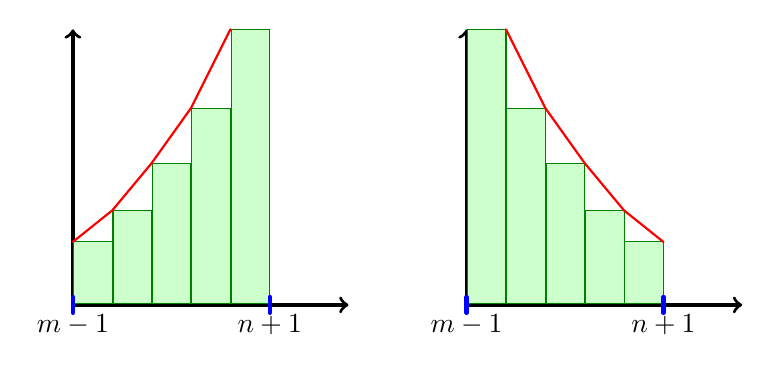
\begin{tikzpicture}
		[scale=1,line cap=round,
		%Styles
		axes/.style=,
		important line/.style={very thick},
		information text/.style={rounded corners,fill=red!10,inner sep=1ex},
		dot/.style={circle,inner sep=1pt,fill,label={#1},name=#1},
		shifted/.style={xshift=5cm}			
		]
		
		%Colors
		\colorlet{anglecolor}{green!50!black}	%angle arcs/lines
		
		%The graphic
		\draw[->,very thick] (0, 0) -- (0, 3.5);
		\draw[->,very thick] (0, 0) -- (3.5, 0);
		
		\filldraw[draw=anglecolor,fill=green!20] (.01,.02) rectangle (.5, .8);
		\filldraw[draw=anglecolor,fill=green!20] (.51, .02) rectangle (1,1.2);
		\filldraw[draw=anglecolor,fill=green!20] (1.01, .02) rectangle (1.5,1.8);
		\filldraw[draw=anglecolor,fill=green!20] (1.51, .02) rectangle (2,2.5);
		\filldraw[draw=anglecolor,fill=green!20] (2.01, .02) rectangle (2.5,3.5);
		
		\draw[red,thick] (0, .8) -- (.5, 1.2) -- (1, 1.8) -- (1.5, 2.5) -- (2, 3.5);
		
		\node[black,below] at (0,0) {$m-1$};
		\node[black,below] at (2.5,0) {$n+1$};
		
		\draw[blue,ultra thick] (0,.1) -- (0, -.1);
		\draw[blue,ultra thick] (2.5,.1) -- (2.5, -.1);
		
		\begin{scope}[xshift=5cm]
			\draw[->,very thick] (0, 0) -- (0, 3.5);
			\draw[->,very thick] (0, 0) -- (3.5, 0);
			
			\filldraw[draw=anglecolor,fill=green!20] (.01,.02) rectangle (.5, 3.5);
			\filldraw[draw=anglecolor,fill=green!20] (.51, .02) rectangle (1,2.5);
			\filldraw[draw=anglecolor,fill=green!20] (1.01, .02) rectangle (1.5,1.8);
			\filldraw[draw=anglecolor,fill=green!20] (1.51, .02) rectangle (2,1.2);
			\filldraw[draw=anglecolor,fill=green!20] (2.01, .02) rectangle (2.5,.8);
			
			\draw[red,thick] (.5, 3.5) -- (1, 2.5) -- (1.5, 1.8) -- (2, 1.2) -- (2.5, .8);
			
			\node[black,below] at (0,0) {$m-1$};
			\node[black,below] at (2.5, 0) {$n+1$};
			
			\draw[blue,ultra thick] (0,.1) -- (0, -.1);
			\draw[blue,ultra thick] (2.5,.1) -- (2.5, -.1);
		\end{scope}
	\end{tikzpicture}
	\end{center}
	
	For an increasing $f$,
	\begin{equation}
		\int_{m-1}^n f(x)dx \leq \sum_{i=m}^n f(i) \leq \sum_m^{n+1} f(x)dx
	\end{equation}
	and for a decreasing $f$,
	\begin{equation}
		\int_{m}^{n+1} f(x)dx \leq \sum_{i=m}^{n} f(i) \leq \int_{m-1}^n f(x)dx
	\end{equation}

%	\begin{figure}[htb]
%		\centering
%		\includegraphics[width=0.8\textwidth]{filename.eps}
%		\caption{Caption.}
%		\label{fig:figure}
%	\end{figure}
	
%	\begin{center}
%	\begin{tikzpicture}
%		[scale=3,line cap=round,
%		%Styles
%		axes/.style=,
%		important line/.style={very thick},
%		information text/.style={rounded corners,fill=red!10,inner sep=1ex},
%		dot/.style={circle,inner sep=1pt,fill,label={#1},name=#1}			
%		]
%		
%		%Colors
%		\colorlet{anglecolor}{green!50!black}	%angle arcs/lines
%		
%		%The graphic
%	\end{tikzpicture}
%	\end{center}

%	\begin{figure}[htb]
%		\centering
%		\includegraphics[width=0.8\textwidth]{filename.eps}
%		\caption{Caption.}
%		\label{fig:figure}
%	\end{figure}

%		\def\enotesize{\normalsize}
%		\theendnotes
\end{document}